%%%%%%%%%%%%%%%%%%%%%%%%%%%%%%%%%%%%%%%%%%%%%%%%%%%%%%%%%%%%%%%%%%%%
%% I, the copyright holder of this work, release this work into the
%% public domain. This applies worldwide. In some countries this may
%% not be legally possible; if so: I grant anyone the right to use
%% this work for any purpose, without any conditions, unless such
%% conditions are required by law.
%%%%%%%%%%%%%%%%%%%%%%%%%%%%%%%%%%%%%%%%%%%%%%%%%%%%%%%%%%%%%%%%%%%%

\documentclass[aspectratio=169, usenames,dvipsnames]{beamer}
% \usefonttheme[onlymath]{serif}
\usetheme[faculty=fi]{fibeamer}
\usepackage[utf8]{inputenc}
\usepackage[spanish]{babel}
\usepackage{environ}
\usepackage{tcolorbox}
\usepackage{xcolor}
\usepackage{transparent}
\usepackage{emoji}
\usepackage{tikz}
\usepackage{listings}

% \usefonttheme[onlymath]{serif}
\definecolor{opagreen}{RGB}{74, 95, 72}
\definecolor{opared}{RGB}{100, 46, 44}
\definecolor{opablue}{RGB}{29,84, 105}
\definecolor{bg}{HTML}{2B2E34}



%% These macros specify information about the presentation
\title{Cuadrados mínimos}
\subtitle{Laboratorio de Datos, IC - FCEN - UBA - 1er. Cuatrimestre 2024}
\author{}

\usepackage{graphicx}

%% These additional packages are used within the document:
\usepackage{ragged2e}  % `\justifying` text
\usepackage{booktabs}  % Tables
\usepackage{tabularx}
\usepackage{tikz}      % Diagrams
\usepackage{tkz-graph}
\usepackage{amsmath, amsfonts, amssymb}
\usetikzlibrary{calc, shapes, backgrounds, decorations.markings}
\DeclareMathOperator*{\argmin}{arg\,min}
\usepackage{url}       % `\url`s
\usepackage{listings}  % Code listings
\newcommand{\dsum}{\displaystyle\sum}

\usefonttheme{professionalfonts} % required for mathspec
% \usepackage{mathspec}
% \setsansfont[BoldFont={Fira Sans},
% Numbers={OldStyle}]{Fira Sans Light}
% \setmathsfont(Digits)[Numbers={Lining, Proportional}]{Fira
% Sans Light}

\begin{document}

%   \shorthandoff{-}
  \frame[c]{\maketitle}

%   \AtBeginSection[]{% Print an outline at the beginning of sections
%     \begin{frame}<beamer>
%       \frametitle{Outline for Section \thesection}
%       \tableofcontents[currentsection]
%     \end{frame}}


  \AtBeginSection[]{% Print an outline at the beginning of sections
    \begin{frame}<beamer>
    \vfill
    \centering
    \Huge{\insertsectionhead}
    \vfill
    \end{frame}}

\section{Cuadrados Mínimos}

\begin{frame}
    \centering
    Teníamos los datos del precio de Bitcoin durante cierto periodo
    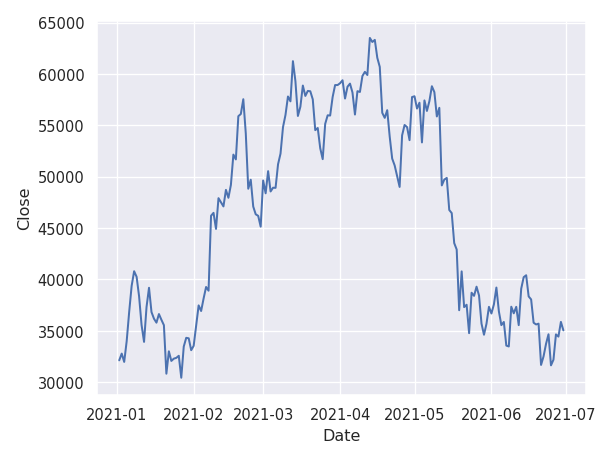
\includegraphics[width=0.7\textwidth]{img/bitcoin.png}
\end{frame}

\begin{frame}
    \centering
    El ajuste lineal no explica muy bien la evolución del precio...
    \begin{columns}
        \begin{column}{0.7\textwidth}
        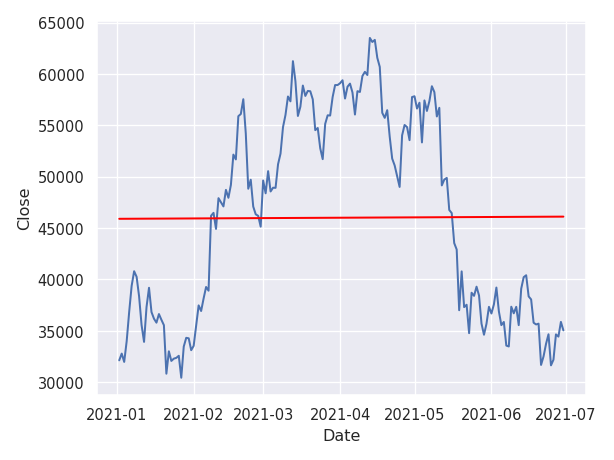
\includegraphics[width=\textwidth]{img/bitcoin_lr.png}
        \end{column}
        \begin{column}{0.3\textwidth}
        $Y = 45900 + 1.18 X$
        $R^2 \approx 3.81 \times 10^{-5}$

        \vspace{2em}
        Obs: el promedio del precio en este periodo fue de U\$D46005
        \end{column}
    \end{columns}
\end{frame}

\begin{frame}
    Cuando la recta no ajusta bien a los datos, podemos intentar ajustarlos con un \textbf{polinomio} de grado más grande.

    \vspace{2em}
    \textbf{Recordemos:} polinomio de grado $n$
    \[ Y = \beta_0 + \beta_1 X + \beta_2 X^2 + \beta_3 X^3 + \dots + \beta_n X^n\]
\end{frame}

\begin{frame}
    Supongamos que queremos aproximar los datos con un polinomio de grado \textit{a lo sumo} $5$:
    \[P(x) = \beta_0 + \beta_1 x + \beta_2 x^2 + \beta_3 x^3 + \beta_4 x^4 + \beta_5 x^5 \]

    \pause
    Tal cual hicimos con regresión lineal, queremos encontrar los valores de $\beta_0, \beta_1, \beta_2, \beta_3, \beta_4, \beta_5$ que minimicen los residuos:
    \[y_i - P(x_i)\]
\end{frame}

\begin{frame}
    Para minimizar los residuos, podemos usar \textbf{Cuadrados Mínimos}. Es decir, \underline{igual que hicimos con Regresión Lineal}, queremos encontrar los $\beta$ que minimicen la suma de los cuadrados de los residuos:
    \[RSS(\beta) = \displaystyle\sum_{i=1}^n (y_i - P(x_i))^2\]

    \pause
    \vspace{1em}
    Las medidas de desempeño del modelo son análogas a las de Regresión Lineal:
    \vspace{0.5em}
    \begin{columns}
        \begin{column}{0.5\textwidth}
            \[R^2 = \dfrac{\sum_{i=1}^n (P(x_i) - \bar{y})^2}{\sum_{i=1}^n (y_i - \bar{y})^2}\]
        \end{column}
        \begin{column}{0.5\textwidth}
            \[ECM = \dfrac{1}{n}\sum_{i=1}^n (y_i - P(x_i))^2\]
        \end{column}

    \end{columns}
\end{frame}

\begin{frame}
    Si todo viene siendo muy parecido a Regresión Lineal, entonces deben haber fórmulas \textit{sencillas} para calcular cada $\beta$...

    \vspace{2em}
    \pause
    Si bien al buscar los mínimos de $RSS(\beta)$ también se obtiene un sistema de ecuaciones lineales, para calcular el valor de los $\beta$ necesitamos herramientas que se ven en \alert{Álgebra Lineal Computacional}.

    \vspace{2em}

    Sin embargo, gracias a \texttt{seaborn}, la visualización es sencilla:
\end{frame}

\begin{frame}
    \centering
    \texttt{.add(so.Line(color='red'), so.PolyFit(1))}
    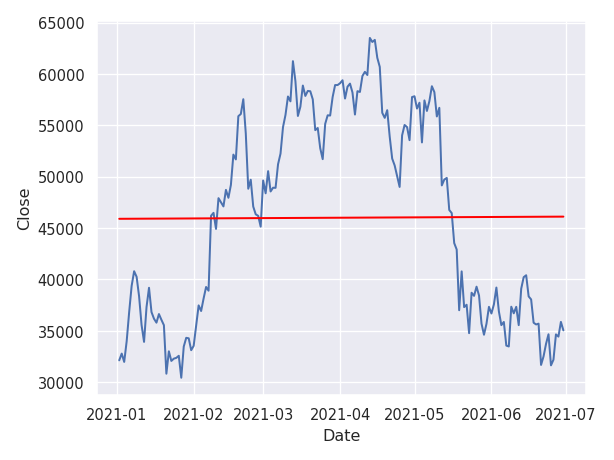
\includegraphics[width=0.75\linewidth]{img/bitcoin_lr.png}
\end{frame}

\begin{frame}
    \centering
    \texttt{.add(so.Line(color='red'), so.PolyFit(\alert{5}))}
    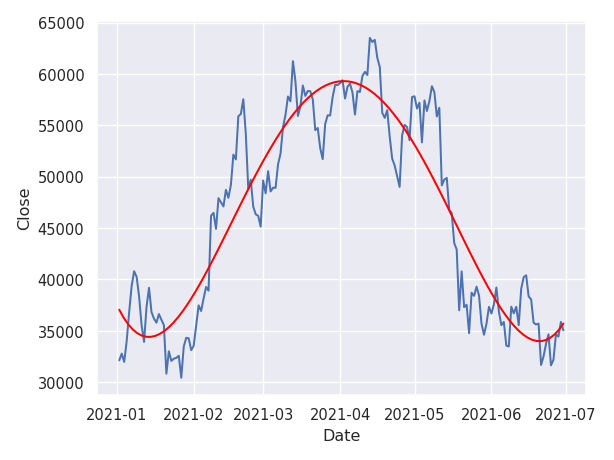
\includegraphics[width=0.75\linewidth]{img/bitcoin_lsq.png}
    \begin{tikzpicture}[remember picture,overlay]
        \node[xshift=3cm, yshift=1cm] at (current page.west) {
\includegraphics[scale=0.15]{img/meme_04.jpg}};
    \end{tikzpicture}
\end{frame}

\begin{frame}
    \Large
    ¿Cómo elegimos el grado del polinomio?

    \normalsize
    El grado del polinomio es el \underline{parámetro} del modelo. No hay una fórmula o una regla que nos diga cuál es el grado apropiado para nuestros datos. 
    
    \pause
    Sin embargo, tenemos algunas opciones:
    \begin{itemize}
        \item dividir nuestros datos en un conjunto de entrenamiento y en uno de testeo para probar cuál es el grado que mejor se desempeña.
        \item tener algún conocimiento específico respecto a nuestros datos.
    \end{itemize}

    \pause
    \alert{\textbf{Obs:} a mayor grado, más complejo es el modelo y mayores son los riesgos de \textit{overfitting} y de tener un problema \textit{mal condicionado}.}
\end{frame}

\section{Bonus: Aplicación de Regresión Lineal}

\begin{frame}
    \centering
    \Large
    Media Movil de Cuadrados Minimos
    
    \normalsize
    Least Squares Moving Average (LSMA)

    \pause
    
\includegraphics[scale=0.4]{img/meme_05.jpg}
\end{frame}

\begin{frame}
    
        En el mercado bursátil, la LSMA es utilizada como un \underline{indicador}:
        
        \begin{itemize}
            \item "Suaviza'' el movimiento del precio del activo por lo que captura mejor la \textbf{tendencia}. \alert{No tiene como objetivo predecir el precio.}
            \item Temporalmente, se mueve un poco por detrás del precio del activo (\textit{lag}).
            \item El cruce de dos LSMA de distintos periodos puede ser una señal de compra o de venta.
        \end{itemize}
\end{frame}

\begin{frame}
    \Large
    ¿Cómo calculamos la LSMA?

    \normalsize
    Supongamos que tenemos nuestros datos $\{(x_1, y_1), (x_2, y_2), \dots, (x_n, y_n)\}$

    \vspace{1em}
    Lo primero que hay que hacer es fijar un periodo de tiempo $k$.

    \vspace{1em}
    Notamos como $\hat{y}_i$ a la estimación de LSMA para $x_i$ y se calcula de la siguiente manera:
    \[\hat{y}_i = \beta_0 + \beta_1 x_i \]
    donde $\beta_0$ y $\beta_1$ son los coeficientes de la \textbf{Regresión Lineal sobre los anteriores $k$ datos:} 
    \[\{(x_{i-k-1}, y_{i-k-1}), (x_{i-k}, y_{i-k}), \dots, (x_{i-1}, y_{i-1})\}\]
\end{frame}

\begin{frame}
    \centering
\only<1>{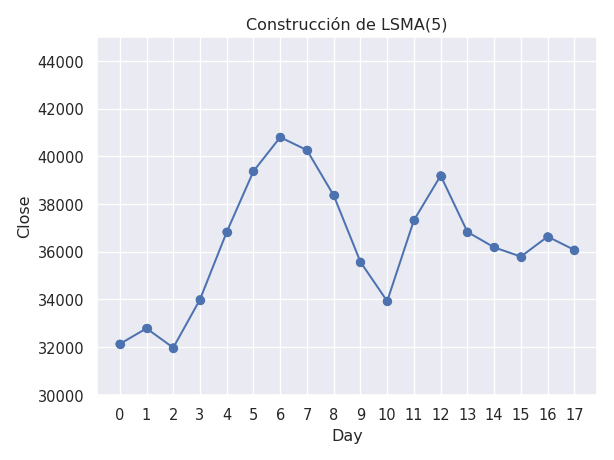
\includegraphics[scale=0.75]{img/LSMA_0.png}}
\only<2>{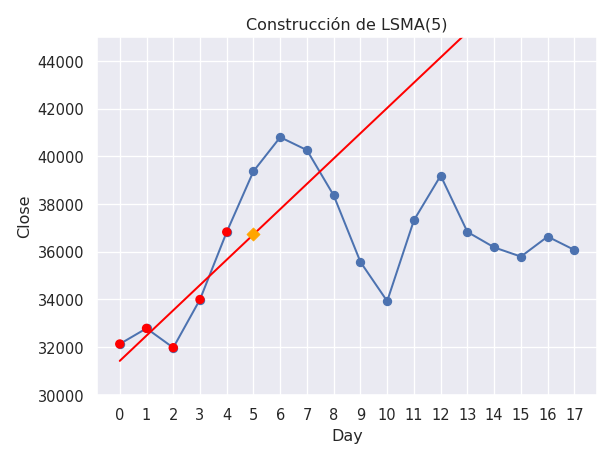
\includegraphics[scale=0.75]{img/LSMA_1.png}}
\only<3>{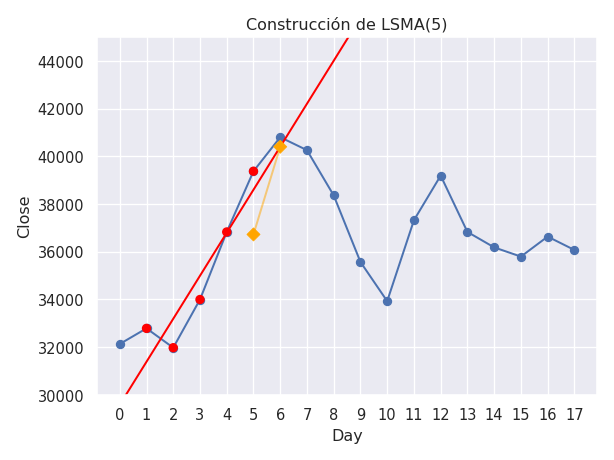
\includegraphics[scale=0.75]{img/LSMA_2.png}}
\only<4>{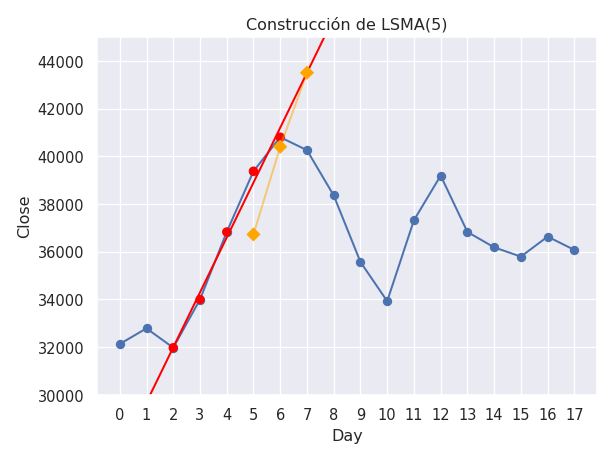
\includegraphics[scale=0.75]{img/LSMA_3.png}}
\only<5>{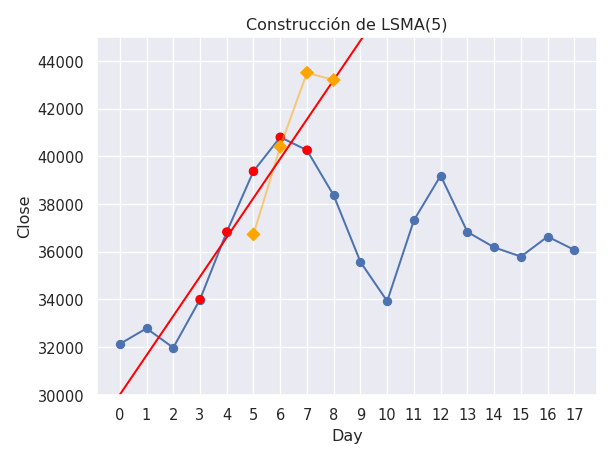
\includegraphics[scale=0.75]{img/LSMA_4.png}}
\only<6>{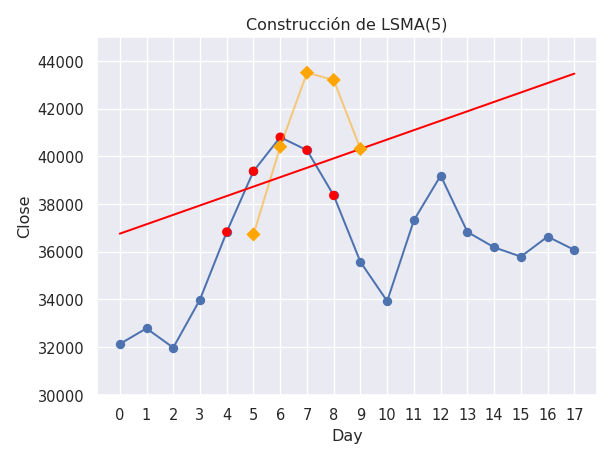
\includegraphics[scale=0.75]{img/LSMA_5.png}}
\only<7>{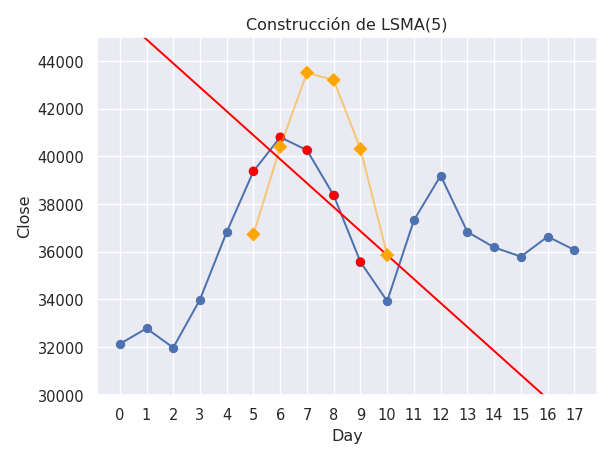
\includegraphics[scale=0.75]{img/LSMA_6.png}}
\only<8>{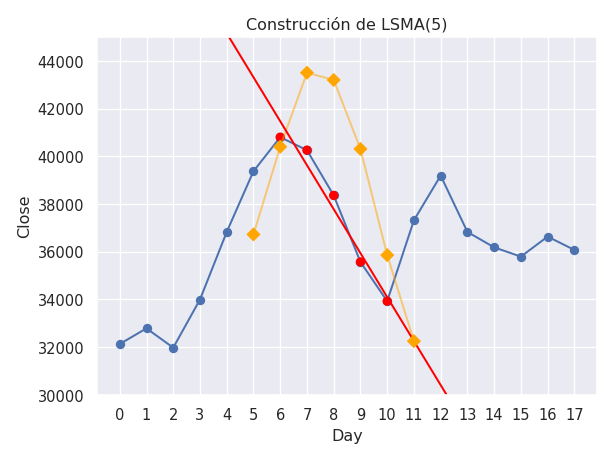
\includegraphics[scale=0.75]{img/LSMA_7.png}}
\only<9>{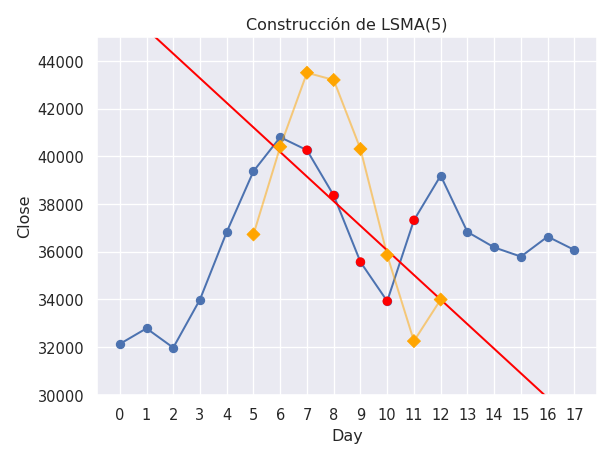
\includegraphics[scale=0.75]{img/LSMA_8.png}}
\only<10>{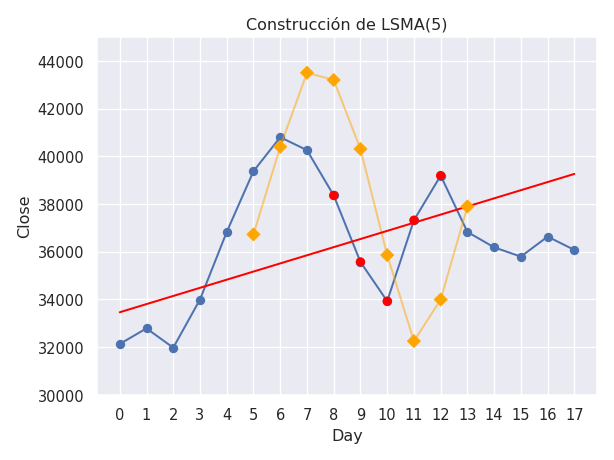
\includegraphics[scale=0.75]{img/LSMA_9.png}}
\only<11>{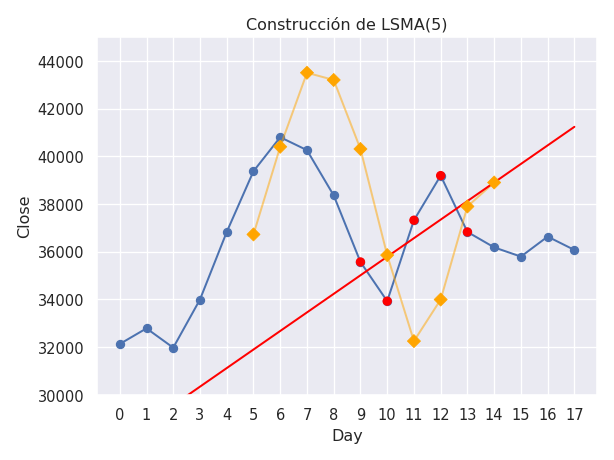
\includegraphics[scale=0.75]{img/LSMA_10.png}}
\only<12>{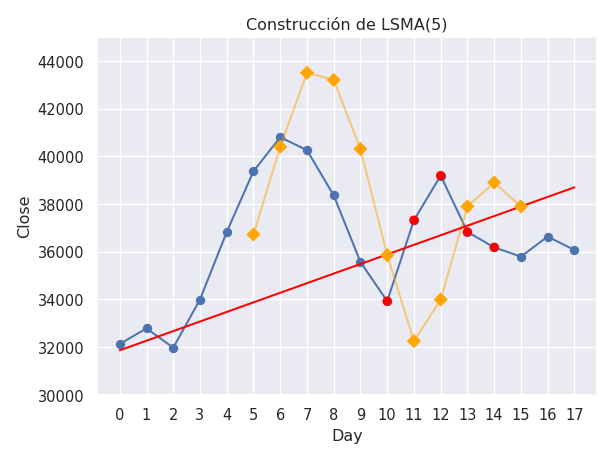
\includegraphics[scale=0.75]{img/LSMA_11.png}}
\only<13>{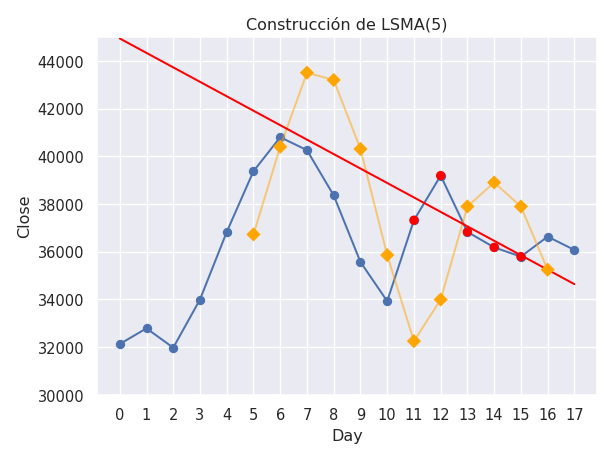
\includegraphics[scale=0.75]{img/LSMA_12.png}}
\only<14>{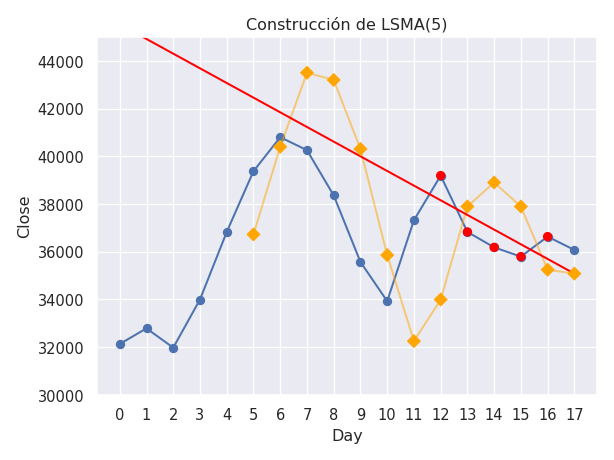
\includegraphics[scale=0.75]{img/LSMA_13.png}}
\only<15>{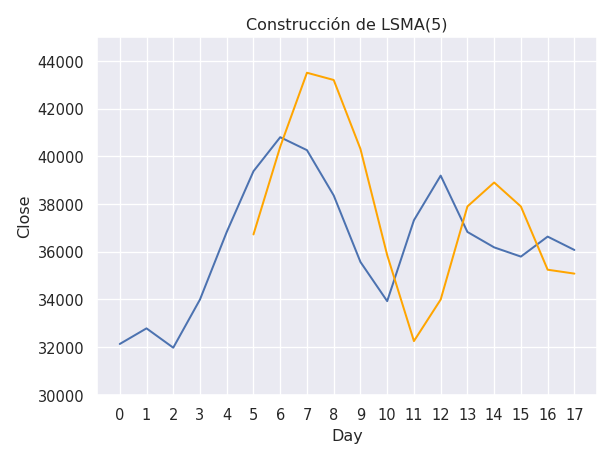
\includegraphics[scale=0.75]{img/LSMA_14.png}}
\end{frame}
\end{document}

